% !TeX program = lualatex
% ================================================================
% Polish Parallel Text Version of PureRatioCrossTopics
%
% Generated by the server using the following settings:
%
%   language            Polish (pol)
%   text direction      left to right
%   font                Noto Serif
%   fallback font       Noto Serif
%   built from          latex/worksheets/ratioAndProportion/crossTopic/pureRatioCrossTopics.tex
%   vocabulary key      latex/worksheets/ratioAndProportion/crossTopic/pureRatioCrossTopics/L2/pol/pureRatioCrossTopics_polishKey.tex
%   tier 3 vocabulary   green   RGB 0 128 0
%   English text        black   RGB 0 0 0
%   Polish text         purple  RGB 112 48 160
%   layout macros       version 3
%
% Please don't edit any information in this comment block - the server
% compares it against the current settings and rebuilds this file when
% they differ, so changes here would be overwritten. However, feel free
% to make updates to the LaTeX below if you want to edit it.
% ================================================================

\documentclass[12pt,a4paper]{article}
% ================================================================
% Copied from the English sheet this was translated from, so that
% anything it sets up for itself still works here
% ================================================================
\usepackage{amsmath} % For advanced math formatting
\usepackage{enumitem} % For customising lists
\usepackage{tikz} % For drawing diagrams
\usepackage{geometry} % For adjusting page margins
\geometry{margin=1in}

\title{Ratio Extension Problems}
\date{}

% Characters this language's font has not got are borrowed from another,
% rather than being silently dropped - see docs/translated-sheet-latex.md
\directlua{%
  if luaotfload and luaotfload.add_fallback then
    luaotfload.add_fallback("eallatinfallback",
      { "Noto Serif:mode=harf;" })
  else
    tex.error("this luaotfload is too old to register a fallback font")
  end
}
\usepackage[english]{babel}
\babelprovide[import]{polish}
\babelfont[polish]{rm}[Renderer=Harfbuzz, BoldFont={Noto Serif}, ItalicFont={Noto Serif}, BoldItalicFont={Noto Serif}, RawFeature={fallback=eallatinfallback}]{Noto Serif}
\babelfont[polish]{sf}[Renderer=Harfbuzz, BoldFont={Noto Serif}, ItalicFont={Noto Serif}, BoldItalicFont={Noto Serif}, RawFeature={fallback=eallatinfallback}]{Noto Serif}
\newcommand{\ealtext}[1]{\foreignlanguage{polish}{#1}}
\newcommand{\ealtextblock}[1]{{\raggedright\foreignlanguage{polish}{#1}\par}}
% ================================================================
% EAL layout helpers
% ================================================================
\usepackage{xcolor}

\definecolor{ealkeycolour}{RGB}{0,128,0}
\definecolor{ealenglish}{RGB}{0,0,0}
\definecolor{ealtwocolour}{RGB}{112,48,160}

\newsavebox{\ealboxen}
\newsavebox{\ealboxtr}
\newlength{\ealglosswd}
\newlength{\ealglossraise}
\setlength{\ealglossraise}{1.15em}

% a tier 3 word, in English and in translation alike
\newcommand{\ealkey}[1]{\textcolor{ealkeycolour}{#1}}
\newcommand{\ealkeytr}[1]{\textcolor{ealkeycolour}{\ealtext{#1}}}

% One translated word above one English word. Built from kernel
% primitives, never a tabular, which would break wherever the sheet
% loads array, booktabs or tabularx. The box is as wide as the wider of
% the two, so a long translation pushes its neighbours aside instead of
% overlapping them, and it claims its full height so a table row or a
% TikZ node makes room for it.
\newcommand{\ealgloss}[2]{%
  \sbox{\ealboxen}{\ealkey{#1}}%
  \sbox{\ealboxtr}{\small\textcolor{ealtwocolour}{\ealtext{#2}}}%
  \setlength{\ealglosswd}{\wd\ealboxen}%
  \ifdim\wd\ealboxtr>\ealglosswd\setlength{\ealglosswd}{\wd\ealboxtr}\fi
  \leavevmode
  \makebox[\ealglosswd][c]{%
    \makebox[0pt][c]{\usebox{\ealboxen}}%
    \makebox[0pt][c]{\raisebox{\ealglossraise}{\usebox{\ealboxtr}}}%
  }%
}

% opens up line spacing around a block of glosses, so the raised
% translations sit clear of the line above
\newenvironment{ealglossed}{\par\linespread{2.1}\selectfont\ignorespaces}{\par}

% a whole translated sentence above its English counterpart. block level,
% so it does not belong inside a tabular cell
\newcommand{\ealpara}[2]{%
  \par\addvspace{0.5\baselineskip}%
  {\color{ealtwocolour}\ealtextblock{#1}}%
  \penalty200
  {\color{ealenglish}#2\par}%
  \addvspace{0.5\baselineskip}%
}

\begin{document}

\maketitle

\section*{\ealkey{Simplifying} \ealkey{Ratios} Past}
\ealpara{\ealkeytr{Uprość} następujące \ealkeytr{stosunki}. Niektóre pytania wymagają najpierw pracy z \ealkeytr{procentami}.}{\emph{\ealkey{Simplify} the following \ealkey{ratios}. Some questions involve working with \ealkey{percentages} first.}}

\begin{enumerate}
\item \ealpara{W badaniu 60\% osób wolało herbatę, a 40\% kawę. Zapisz \ealkeytr{stosunek} osób pijących herbatę do osób pijących kawę w \ealkeytr{najprostszej postaci}.}{In a survey, 60\% of people preferred tea and 40\% preferred coffee. Write the \ealkey{ratio} of tea drinkers to coffee drinkers in its \ealkey{simplest form}.}

\vspace{1.2cm}

\item \ealpara{Koszula jest przeceniona o 30\%. Kwota rabatu wynosi £12. Jaki jest \ealkeytr{stosunek} kwoty rabatu do ceny pierwotnej? \ealkeytr{Uprość} swoją odpowiedź.}{A shirt is on sale for 30\% off. The discount amount is £12. What is the \ealkey{ratio} of the discount amount to the original price? \ealkey{Simplify} your answer.}

\vspace{1.2cm}

\item \ealpara{Bateria straciła 15\% swojego naładowania. Jaki jest \ealkeytr{stosunek} utraconego naładowania do pozostałego naładowania? \ealkeytr{Uprość} swoją odpowiedź.}{A battery has lost 15\% of its charge. What is the \ealkey{ratio} of the charge lost to the charge remaining? \ealkey{Simplify} your answer.}

\vspace{1.2cm}

\item \ealpara{W ciągu roku zyski firmy podzielono następująco: 45\% zainwestowano ponownie, 20\% wypłacono jako dywidendy, a resztę przeznaczono na premie dla pracowników.}{In a year, a company's profits were allocated as follows: 45\% was reinvested, 20\% was paid as dividends, and the rest was used for employee bonuses.}
    \begin{enumerate}
    \item \ealpara{Jaki \ealkeytr{procent} przeznaczono na premie dla pracowników?}{What \ealkey{percentage} was used for employee bonuses?}
    \item \ealpara{Wyraź \ealkeytr{stosunek} Reinwestycja : Dywidendy : Premie w \ealkeytr{najprostszej postaci}.}{Express the \ealkey{ratio} Reinvestment : Dividends : Bonuses in its \ealkey{simplest form}.}
    \end{enumerate}

\vspace{1.2cm}

\item \ealpara{Populacja miasteczka wynosi 12,500. Po spisie ludności okazuje się, że populacja wzrosła o 18\%. Jaki jest \ealkeytr{stosunek} nowej populacji do pierwotnej populacji? Wyraź odpowiedź w postaci \( a : b \), gdzie \( a \) i \( b \) są \ealkeytr{liczbami całkowitymi}.}{The population of a town is 12,500. After a census, it's found that the population has increased by 18\%. What is the \ealkey{ratio} of the new population to the original population? Express your answer in the form \( a : b \), where \( a \) and \( b \) are \ealkey{integers}.}

\end{enumerate}

\newpage{}

\section*{\ealkey{Simplifying} \ealkey{Ratios} Future}
\ealpara{Użyj diagramów, aby pomóc sobie odpowiedzieć na pytania o \ealkeytr{stosunki} \ealkeytr{pól} i \ealkeytr{obwodów}.}{\emph{Use the diagrams to help you answer the questions about the \ealkey{ratios} of \ealkey{areas} and \ealkey{perimeters}.}}

\begin{enumerate}
\setcounter{enumi}{5}
\item \ealpara{Dwa prostokąty poniżej są \ealkeytr{podobne}. Znajdź \ealkeytr{stosunek} \ealkeytr{obwodu} prostokąta A do \ealkeytr{obwodu} prostokąta B. Następnie znajdź \ealkeytr{stosunek} \ealkeytr{pola} prostokąta A do \ealkeytr{pola} prostokąta B.}{The two rectangles below are \ealkey{similar}. Find the \ealkey{ratio} of the \ealkey{perimeter} of rectangle A to the \ealkey{perimeter} of rectangle B. Then, find the \ealkey{ratio} of the \ealkey{area} of rectangle A to the \ealkey{area} of rectangle B.}

\vspace{0.5cm}
\begin{center}
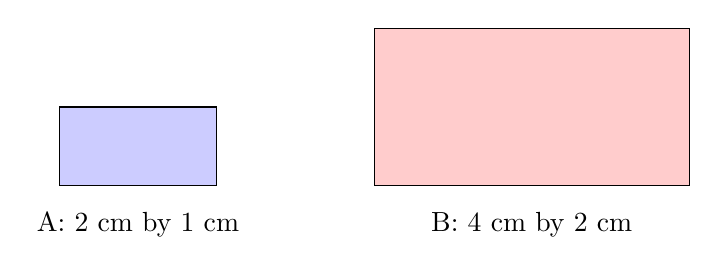
\begin{tikzpicture}
\draw[fill=blue!20] (0,0) rectangle (2,1);
\node at (1, -0.5) {A: 2 cm by 1 cm};
\draw[fill=red!20] (4,0) rectangle (8,2);
\node at (6, -0.5) {B: 4 cm by 2 cm};
\end{tikzpicture}
\end{center}

\vspace{1.2cm}

\item \ealpara{\ealkeytr{Kwadrat} ma bok długości \( s \). Inny \ealkeytr{kwadrat} ma bok długości \( 3s \). Jaki jest \ealkeytr{stosunek} \ealkeytr{obwodu} mniejszego \ealkeytr{kwadratu} do większego \ealkeytr{kwadratu}? Jaki jest \ealkeytr{stosunek} ich \ealkeytr{pól}?}{A \ealkey{square} has a side length of \( s \). Another \ealkey{square} has a side length of \( 3s \). What is the \ealkey{ratio} of the \ealkey{perimeter} of the smaller \ealkey{square} to the larger \ealkey{square}? What is the \ealkey{ratio} of their \ealkey{areas}?}

\vspace{1.2cm}

\item \ealpara{\ealkeytr{Trójkąt prostokątny} ma \ealkeytr{podstawę} 8 cm i \ealkeytr{wysokość} 6 cm. \ealkeytr{Podobny} trójkąt ma \ealkeytr{podstawę} 12 cm.}{A \ealkey{right-angled triangle} has a \ealkey{base} of 8 cm and a \ealkey{height} of 6 cm. A \ealkey{similar} triangle has a \ealkey{base} of 12 cm.}
    \begin{enumerate}
    \item \ealpara{Jaki jest \ealkeytr{współczynnik skali} od mniejszego do większego trójkąta?}{What is the \ealkey{scale factor} from the smaller to the larger triangle?}
    \item \ealpara{Jaki jest \ealkeytr{stosunek} \ealkeytr{obwodu} mniejszego trójkąta do większego trójkąta?}{What is the \ealkey{ratio} of the \ealkey{perimeter} of the smaller triangle to the larger triangle?}
    \item \ealpara{Jaki jest \ealkeytr{stosunek} \ealkeytr{pola} mniejszego trójkąta do większego trójkąta?}{What is the \ealkey{ratio} of the \ealkey{area} of the smaller triangle to the larger triangle?}
    \end{enumerate}

\vspace{1.2cm}

\newpage{}

\item \ealpara{Poniższy diagram pokazuje duży prostokąt z wyciętym z niego mniejszym prostokątem. Znajdź \ealkeytr{stosunek} \ealkeytr{pola} zacieniowanego obszaru do \ealkeytr{pola} niezacieniowanego (wyciętego) prostokąta.}{The diagram below shows a large rectangle with a smaller rectangle cut out of it. Find the \ealkey{ratio} of the \ealkey{area} of the shaded region to the \ealkey{area} of the unshaded (cut-out) rectangle.}

\vspace{0.5cm}
\begin{center}
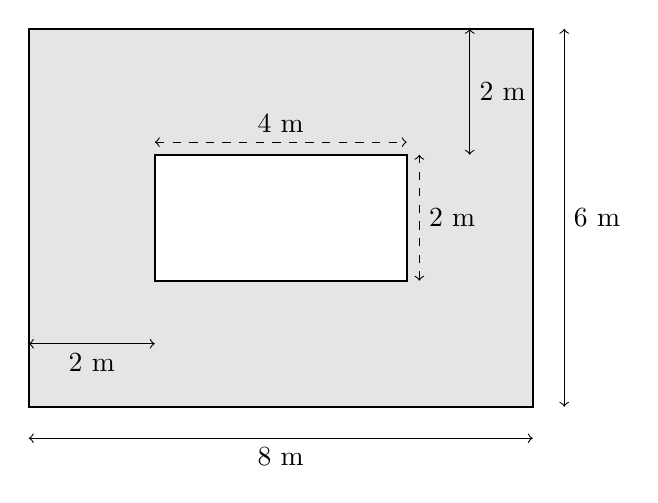
\begin{tikzpicture}[scale=0.8]
    % Big rectangle (shaded region)
    \fill[gray!20] (0,0) rectangle (8,6);
    \draw[thick] (0,0) rectangle (8,6);
    
    % Small rectangle (cut-out) - drawn with thicker white border to show cut-out effect
    \fill[white] (2,2) rectangle (6,4);
    \draw[thick, white] (2,2) rectangle (6,4);
    \draw[thick] (2,2) rectangle (6,4);
    
    % Labels for dimensions
    % Outer rectangle dimensions
    \draw[<->] (0,-0.5) -- (8,-0.5) node[midway,below] {8 m};
    \draw[<->] (8.5,0) -- (8.5,6) node[midway,right] {6 m};
    
    % Inner rectangle positioning dimensions
    \draw[<->] (0,1) -- (2,1) node[midway,below] {2 m};
    \draw[<->] (7,4) -- (7,6) node[midway,right] {2 m};
    
       
    % Inner rectangle dimensions
    \draw[<->, dashed] (2,4.2) -- (6,4.2) node[midway,above] {4 m};
    \draw[<->, dashed] (6.2,2) -- (6.2,4) node[midway,right] {2 m};
\end{tikzpicture}
\end{center}
\ealpara{(\ealkeytr{Wymiary}: duży prostokąt ma 8 m na 6 m. Niezacieniowany prostokąt ma długość 4 m i jest umieszczony centralnie.)}{\textit{(\ealkey{Dimensions}: Large rectangle is 8m by 6m. The unshaded rectangle has a length of 4m and is positioned centrally.)}}

\vspace{1.2cm}

\item \ealpara{Okrągły staw ma \ealkeytr{promień} \( r \). Wokół niego zbudowano ścieżkę, tworząc większy okrąg o \ealkeytr{promieniu} \( R \), gdzie \( R = 2r \).}{A circular pond has a \ealkey{radius} of \( r \). A path is built around it, creating a larger circle with a \ealkey{radius} of \( R \), where \( R = 2r \).}
    \begin{enumerate}
    \item \ealpara{Znajdź \ealkeytr{stosunek} \ealkeytr{obwodu} stawu do \ealkeytr{obwodu} zewnętrznej krawędzi ścieżki.}{Find the \ealkey{ratio} of the \ealkey{circumference} of the pond to the \ealkey{circumference} of the outer edge of the path.}
    \item \ealpara{Znajdź \ealkeytr{stosunek} \ealkeytr{pola} stawu do całkowitego \ealkeytr{pola} ograniczonego zewnętrzną krawędzią ścieżki.}{Find the \ealkey{ratio} of the \ealkey{area} of the pond to the total \ealkey{area} enclosed by the outer edge of the path.}
    \end{enumerate}

\vspace{1.2cm}
\end{enumerate}

\section*{Sharing Into \ealkey{Ratios} Past}
\ealpara{Podziel podane ilości w podanych \ealkeytr{stosunkach}, wykorzystując informacje o \ealkeytr{procencie}, aby ci pomóc.}{Share the given quantities in the specified \ealkey{ratios}, using the \ealkey{percentage} information to help you.}

\begin{enumerate}
    \setcounter{enumi}{10}
    \item \ealpara{Suma £80 jest dzielona między dwie osoby. Osoba A otrzymuje 60\% całości. Jaki jest \ealkeytr{stosunek} ich udziałów i ile otrzymuje każda osoba?}{A sum of £80 is shared between two people. Person A receives 60\% of the total. What is the \ealkey{ratio} of their shares, and how much does each person receive?}
    
    \item \ealpara{W klasie 40\% uczniów to chłopcy, a reszta to dziewczęta. Fundusz szkolny w wysokości £150 ma być podzielony między chłopców i dziewczęta w takim samym \ealkeytr{stosunku} jak ich liczby w klasie. Ile dostaną chłopcy?}{In a class, 40\% of students are boys and the rest are girls. The school fund of £150 is to be shared between boys and girls in the same \ealkey{ratio} as their numbers in the class. How much do the boys get?}
    
    \item \ealpara{Premia w wysokości £2,500 jest dzielona między trzy działy w \ealkeytr{proporcjonalności} do ich wkładu w zyski firmy wyrażonego w \ealkeytr{procentach}. Dział A wniósł 25\%, dział B 35\%, a dział C resztę. Ile otrzymuje każdy dział i jaki jest \ealkeytr{stosunek} ich udziałów w \ealkeytr{najprostszej postaci}?}{A bonus of £2,500 is shared between three departments in \ealkey{proportion} to their \ealkey{percentage} contribution to company profits. Department A contributed 25\%, Department B 35\%, and Department C the remainder. How much does each department receive, and what is the \ealkey{ratio} of their shares in \ealkey{simplest form}?}
    
    \item \ealpara{W przepisie suche składniki (mąka i cukier) są mieszane w \ealkeytr{stosunku} 3:2 według masy. Jeśli mąka stanowi 30\% całej mieszanki (w tym 400 g mokrych składników), znajdź masę użytej mąki i cukru.}{In a recipe, the dry ingredients (flour and sugar) are mixed in the \ealkey{ratio} 3:2 by weight. If the flour makes up 30\% of the total mixture (including 400g of wet ingredients), find the weight of flour and sugar used.}
    
    \item \ealpara{Spadek jest dzielony między troje dzieci. Najstarsze otrzymuje 50\% całości, średnie dziecko otrzymuje 40\% tego, co otrzymuje najstarsze, a najmłodsze otrzymuje pozostałe £24,000. Znajdź całkowity spadek i \ealkeytr{stosunek} ich udziałów w postaci \textit{Najstarsze : Średnie : Najmłodsze}.}{An inheritance is shared between three children. The eldest receives 50\% of the total, the middle child receives 40\% of what the eldest gets, and the youngest receives the remaining £24,000. Find the total inheritance and the \ealkey{ratio} of their shares in the form \textit{Eldest : Middle : Youngest}.}
\end{enumerate}

\section*{Sharing Into \ealkey{Ratios} Future}
\ealpara{Użyj diagramów, aby pomóc sobie rozwiązać następujące zadania.}{Use the diagrams to help you solve the following problems.}

\begin{enumerate}
    \setcounter{enumi}{15}
    \item \ealpara{\ealkeytr{Obwód} prostokąta wynosi 30 cm. Boki są w \ealkeytr{stosunku} 2:3. Znajdź \ealkeytr{pole} prostokąta.}{The \ealkey{perimeter} of a rectangle is 30 cm. The sides are in the \ealkey{ratio} 2:3. Find the \ealkey{area} of the rectangle.}
    
    \item \ealpara{\ealkeytr{Pole} prostokąta wynosi 54 cm². Boki są w \ealkeytr{stosunku} 2:3. Znajdź \ealkeytr{obwód} prostokąta.}{The \ealkey{area} of a rectangle is 54 cm². The sides are in the \ealkey{ratio} 2:3. Find the \ealkey{perimeter} of the rectangle.}
    
    \item \ealpara{\ealkeytr{Trójkąt prostokątny} ma boki w \ealkeytr{stosunku} 3:4:5. \ealkeytr{Pole} trójkąta wynosi 96 cm². Znajdź \ealkeytr{obwód} trójkąta.}{A \ealkey{right-angled triangle} has sides in the \ealkey{ratio} 3:4:5. The \ealkey{area} of the triangle is 96 cm². Find the \ealkey{perimeter} of the triangle.}
    
    \begin{tikzpicture}
        \draw (0,0) -- (4,0) -- (0,3) -- cycle;
        \node at (2, -0.3) {?};
        \node at (-0.3, 1.5) {?};
        \node at (2, 1.8) {?};
    \end{tikzpicture}

    \item \ealpara{Ogród ma kształt litery L złożony z dwóch prostokątów. Pierwszy prostokąt ma boki 3 m i 2 m. Drugi prostokąt ma boki w \ealkeytr{stosunku} 3:4. Jeśli całkowite \ealkeytr{pole} ogrodu wynosi 54 m², znajdź \ealkeytr{wymiary} drugiego prostokąta.}{A garden is in the shape of an L-shape made from two rectangles. The first rectangle is 3m by 2m. The second rectangle has sides in the \ealkey{ratio} 3:4, If the total \ealkey{area} of the garden is 54 m², find the \ealkey{dimensions} of the second rectangle.}
    
    \begin{tikzpicture}[scale=0.5]
        \draw (0,0) rectangle (3,2);
        \draw (3,0) rectangle (7,4);
        \node at (1.5, -0.5) {3m};
        \node at (-0.55, 1) {2m};
        \node at (5, -0.5) {?};
        \node at (8, 2) {?};
    \end{tikzpicture}

    \newpage{}

    \item \ealpara{Okrągły staw jest otoczony ścieżką. \ealkeytr{Promień} stawu i szerokość ścieżki są w \ealkeytr{stosunku} 2:1. Jeśli całkowite \ealkeytr{pole} (staw + ścieżka) wynosi $99\pi$m², znajdź szerokość ścieżki.}{A circular pond is surrounded by a path. The \ealkey{radius} of the pond and the width of the path are in the \ealkey{ratio} 2:1. If the total \ealkey{area} (pond + path) is $99\pi$m², find the width of the path.}
    
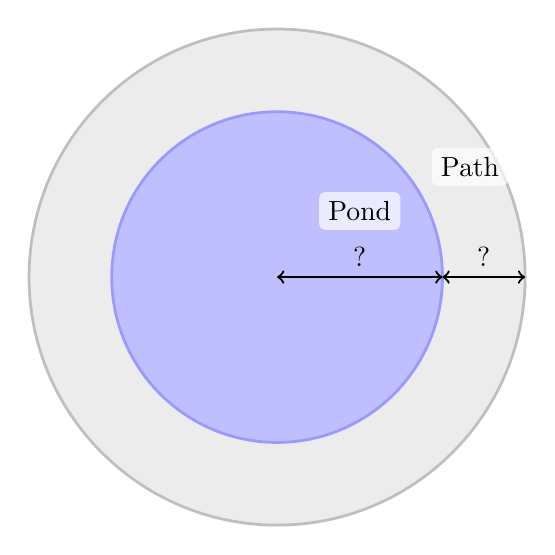
\begin{tikzpicture}[scale=0.7]
    % Path (annulus) - lighter fill with darker border
    \filldraw[fill=gray!15, draw=gray!50, line width=1pt] (0,0) circle (4.5);
    % Pond - darker fill with clear border
    \filldraw[fill=blue!25, draw=blue!40, line width=1pt] (0,0) circle (3);
    
    % Dimension lines with arrows and labels
    \draw[<->, line width=0.8pt] (0,0) -- (3,0) node[midway, above]{?};
    \draw[<->, line width=0.8pt] (3,0) -- (4.5,0) node[midway, above] {?};
    
    % Labels with better positioning and background
    \node[fill=white, fill opacity=0.7, text opacity=1, rounded corners=2pt] at (1.5, 1.2) {Pond};
    \node[fill=white, fill opacity=0.7, text opacity=1, rounded corners=2pt] at (3.5, 2.0) {Path};
    
\end{tikzpicture}
\end{enumerate}

\vspace{1cm}

\section*{\ealkey{Ratio} Problem Solving Past}
\begin{enumerate}[start=21]

    \item \ealpara{W klasie \ealkeytr{stosunek} chłopców do dziewcząt wynosi $3:2$. 40\% chłopców nosi okulary. 20\% dziewcząt nosi okulary, jaki \ealkeytr{procent} \textit{całej klasy} nosi okulary?}{In a class, the \ealkey{ratio} of boys to girls is $3:2$. 40\% of the boys wear glasses. 20\% of the girls wear glasses, what \ealkey{percentage} of the \textit{whole class} wear glasses?}

    \item \ealpara{Cena rzadkiej monety wzrasta o 20\%. Nowy \ealkeytr{stosunek} jej ceny do ceny pierwotnej wynosi $a : b$. Zapisz \ealkeytr{stosunek} $a:b$ w \ealkeytr{najprostszej postaci}.}{The price of a rare coin is increased by 20\%. The new \ealkey{ratio} of its price to its original price is $a : b$. Write the \ealkey{ratio} $a:b$ in its \ealkey{simplest form}.}

    \item \ealpara{Sklep sprzedaje tylko dwa rodzaje owoców: jabłka i pomarańcze. \ealkeytr{Stosunek} jabłek do pomarańczy wynosi $5:3$. 30\% jabłek jest zielonych, a reszta jest czerwona. 60\% pomarańczy pochodzi z Hiszpanii, a reszta z Maroka. Jaki jest \ealkeytr{stosunek} \textbf{zielonych jabłek} do \textbf{pomarańczy z Maroka}?}{A shop sells only two types of fruit: apples and oranges. The \ealkey{ratio} of apples to oranges is $5:3$. 30\% of the apples are green, and the rest are red. 60\% of the oranges are from Spain, and the rest are from Morocco. What is the \ealkey{ratio} of \textbf{green apples} to \textbf{oranges from Morocco}?}

    \item \ealpara{W bibliotece \ealkeytr{stosunek} książek beletrystycznych do literatury faktu wynosi $7:3$. Po darowiźnie liczba książek beletrystycznych wzrosła o 15\%, a liczba książek literatury faktu zmalała o 10\%. Znajdź nowy \ealkeytr{stosunek} książek beletrystycznych do literatury faktu. Podaj odpowiedź w postaci $A:B$, gdzie $A$ i $B$ są \ealkeytr{liczbami całkowitymi}.}{In a library, the \ealkey{ratio} of fiction to non-fiction books is $7:3$. After a donation, the number of fiction books increased by 15\% and the number of non-fiction books decreased by 10\%. Find the new \ealkey{ratio} of fiction to non-fiction books. Give your answer in the form $A:B$ where $A$ and $B$ are \ealkey{integers}.}

    \item \ealpara{Populacja miasteczka wynosi 18,000. \ealkeytr{Stosunek} dorosłych do dzieci wynosi $5:4$. Rok później populacja dorosłych maleje o 5\%, a populacja dzieci wzrasta o 10\%.}{The population of a town is 18,000. The \ealkey{ratio} of adults to children is $5:4$. One year later, the adult population decreases by 5\% and the child population increases by 10\%.}
    \begin{enumerate}[label=(\alph*)]
        \item \ealpara{Jaki jest nowy \ealkeytr{stosunek} dorosłych do dzieci? Podaj odpowiedź w \ealkeytr{najprostszej postaci}.}{What is the new \ealkey{ratio} of adults to children? Give your answer in its \ealkey{simplest form}.}
        \item \ealpara{Jaka jest całkowita zmiana w całkowitej populacji wyrażona w \ealkeytr{procentach}? Podaj odpowiedź z dokładnością do 2 miejsc po przecinku.}{What is the overall \ealkey{percentage} change in the total population? Give your answer to 2 decimal places.}
    \end{enumerate}

\end{enumerate}

\newpage{}

\section*{\ealkey{Ratio} Problem Solving Future}
\begin{enumerate}[start=26]

    \item \ealpara{Dwa prostokąty, A i B, są \ealkeytr{podobne}. \ealkeytr{Stosunek} ich \ealkeytr{odpowiadających} długości wynosi $2:5$. Jaki jest \ealkeytr{stosunek} ich \ealkeytr{obwodów}? Jaki jest \ealkeytr{stosunek} ich \ealkeytr{pól}?}{Two rectangles, A and B, are \ealkey{similar}. The \ealkey{ratio} of their \ealkey{corresponding} lengths is $2:5$. What is the \ealkey{ratio} of their \ealkey{perimeters}? What is the \ealkey{ratio} of their \ealkey{areas}?}

    \item \ealpara{Prostokąt ma \ealkeytr{stosunek} długości do szerokości $5:2$. Jego \ealkeytr{obwód} wynosi 42 cm.}{A rectangle has a length to width \ealkey{ratio} of $5:2$. Its \ealkey{perimeter} is 42 cm.}
    \begin{enumerate}[label=(\alph*)]
        \item \ealpara{Znajdź jego \ealkeytr{pole}.}{Find its \ealkey{area}.}
        \item \ealpara{Jeśli prostokąt jest \ealkeytr{powiększany} przez \ealkeytr{współczynnik skali} 3, jaki jest nowy \ealkeytr{stosunek} długości do szerokości i jakie jest jego nowe \ealkeytr{pole}?}{If the rectangle is \ealkey{enlarged} by a \ealkey{scale factor} of 3, what is the new \ealkey{ratio} of length to width, and what is its new \ealkey{area}?}
    \end{enumerate}

    \item \ealpara{\ealkeytr{Stosunek} \ealkeytr{pola} \ealkeytr{kwadratu} do \ealkeytr{pola} \ealkeytr{trójkąta równobocznego} wynosi $16:9$. \ealkeytr{Obwód} \ealkeytr{kwadratu} wynosi 32 cm. Jaka jest długość jednego boku trójkąta?}{The \ealkey{ratio} of the \ealkey{area} of a \ealkey{square} to the \ealkey{area} of an \ealkey{equilateral triangle} is $16:9$. The \ealkey{perimeter} of the \ealkey{square} is 32 cm. What is the length of one side of the triangle?}

    \item \ealpara{\ealkeytr{Obwód} \ealkeytr{trójkąta równoramiennego} wynosi 36 cm. \ealkeytr{Stosunek} równych boków do \ealkeytr{podstawy} wynosi $5:2$.}{The \ealkey{perimeter} of an \ealkey{isosceles triangle} is 36 cm. The \ealkey{ratio} of the equal sides to the \ealkey{base} is $5:2$.}
    \begin{enumerate}[label=(\alph*)]
        \item \ealpara{Oblicz długości boków trójkąta.}{Calculate the lengths of the sides of the triangle.}
        \item \ealpara{Oblicz \ealkeytr{pole} trójkąta. (Wskazówka: możesz potrzebować \ealkeytr{twierdzenia Pitagorasa} – poproś swojego nauczyciela o pomoc w narysowaniu obrazka!).}{Calculate the \ealkey{area} of the triangle. (Hint: You may need to use \ealkey{Pythagoras' Theorem} - ask your teacher to help you draw a picture!).}
    \end{enumerate}

    \item \ealpara{Poniższy diagram pokazuje duży prostokąt o \ealkeytr{podstawie} 20 cm, z \ealkeytr{podobnym} mniejszym prostokątem o \ealkeytr{wysokości} 4 cm wyciętym z jednego rogu. \ealkeytr{Stosunek} długości do szerokości mniejszego prostokąta jest taki sam jak \ealkeytr{stosunek} długości do szerokości dużego prostokąta.}{The diagram below shows a large rectangle, measuring 20 cm at the \ealkey{base}, with a \ealkey{similar} smaller rectangle, \ealkey{height} 4 cm cut out from one corner. The \ealkey{ratio} of the length to the width of the smaller rectangle is the same as the \ealkey{ratio} of the length to the width of the large rectangle.}
    
    \begin{center}
    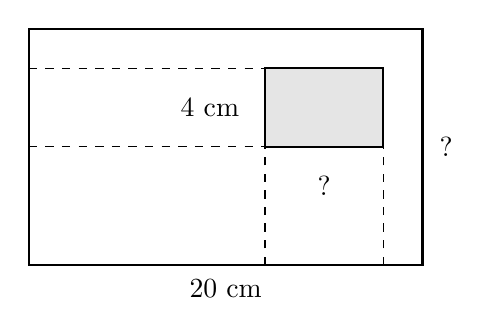
\begin{tikzpicture}
        \draw[thick] (0,0) rectangle (5,3);
        \draw[thick, fill=gray!20] (3,1.5) rectangle (4.5,2.5);
        \draw[dashed] (3,0) -- (3,1.5);
        \draw[dashed] (4.5,0) -- (4.5,1.5);
        \draw[dashed] (0,1.5) -- (3,1.5);
        \draw[dashed] (0,2.5) -- (3,2.5);
        \node at (2.5, -0.3) {20 cm};
        \node at (5.3, 1.5) {?};
        \node at (2.3, 2) {4 cm};
        \node at (3.75, 1) {?};
    \end{tikzpicture}
    \end{center}
    
    \ealpara{Biorąc pod uwagę, że \ealkeytr{pole} dużego prostokąta z wyciętym małym prostokątem wynosi $216 \text{ cm}^2$, znajdź \ealkeytr{wymiary} mniejszego prostokąta.}{Given that the \ealkey{area} of the large rectangle with the small one cut out is $216 \text{ cm}^2$, find the \ealkey{dimensions} of the smaller rectangle.}

\end{enumerate}

\end{document}